\chapter{Specifikacija programske potpore}
		
	\section{Funkcionalni zahtjevi}
			
			
			\noindent \textbf{Dionici:}
			
			\begin{packed_enum}
				
				\item Uprava tvrtke (naručitelj)
				\item Razvojni inženjer				
				\item Voditelj tima
				\item Koordinator timova
				\item Tim koji je razvio aplikaciju
				
			\end{packed_enum}
			
			\noindent \textbf{Aktori i njihovi funkcionalni zahtjevi:}
			
			
			\begin{packed_enum}
				\item  \underbar{Uprava tvrtke (inicijator) može:}
				
				\begin{packed_enum}
					
					\item se prijaviti u sustav
					\item pregledavati napredak bilo kojeg projekta
					
				\end{packed_enum}
			
				\item  \underbar{Zaposlenik (razvojni inženjer/voditelj/koordinator) (inicijator) može:}
				
				\begin{packed_enum}
					
					\item se prijaviti u sustav
					\item pregledavati profil
					\item mijenjati email, korisničko ime i lozinku
					
				\end{packed_enum}
			
				\item  \underbar{Zaposlenik (razvojni inženjer) (inicijator) može:}
			
				\begin{packed_enum}
					
					\item preuzimati zadatke
					\item izvještavati o stanju zadatka
					\item pomicati zadatke kroz faze na kanban ploči
					\item gledati raspored sastanaka s voditeljom
					
				\end{packed_enum}
			
				\item  \underbar{Zaposlenik (voditelj tima) (inicijator) može:}
			
				\begin{packed_enum}
					
					\item dodavati zadatke na backlog
					\item dogovarati sastanke s razvonim inženjerima
					\item preuzimati zadatke
					\item izvještavati o stanju projekta
					\item pomicati zadatke kroz faze na kanban ploči
					\item gledati raspored sastanaka s koordinatorom
					
				\end{packed_enum}
			
				\item  \underbar{Zaposlenik (koordinator) (inicijator) može:}
				
				\begin{packed_enum}
					
					\item stvarati radne skupine
					\item dogovarati sastanke s voditeljima timova
					\item pratiti napredak projekta
					\item izvještavati o stanju projekta
					
				\end{packed_enum}
			
				\item  \underbar{Baza podataka (sudionik):}
				
				\begin{packed_enum}
					
					\item pohranjuje podatke o svim zaposlenicima i njihovim titulama
					\item pohranjuje podatke o svim projektima, zadacima i stanjima zadataka
					
				\end{packed_enum}
			
			\end{packed_enum}
			
			\eject 
			
			
				
			\subsection{Obrasci uporabe}
				
				
				\subsubsection{Opis obrazaca uporabe}

					
	
			
					\noindent \underbar{\textbf{UC1 - Prijava u sustav}}
				\begin{packed_item}
				
					\item \textbf{Glavni sudionik: }Zaposlenik
					\item  \textbf{Cilj:} Pristupiti korisničkom sučelju 
					\item  \textbf{Sudionici:} Baza podataka
					\item  \textbf{Preduvjet:} Korisnik je registriran u bazi 
					\item  \textbf{Opis osnovnog tijeka:}
				
					\item[] \begin{packed_enum}
						
						\item Unos korisničkog imena i lozinke 
						\item Potvrda o ispravnosti unesenih podataka
						\item Pristup korisničkim funkcijama 
					\end{packed_enum}
					\item  \textbf{Opis mogućih odstupanja:} 
				
					\item[] \begin{packed_item}
					
						\item[2.a] Neispravno korisničko ime/lozinka
						\item[] \begin{packed_enum}
						
							\item Sustav obavještava korisnika o neuspjeloj prijavi i vraća ga na stranicu za unos korisničkog imena i lozinke  
						
						\end{packed_enum}
					\end{packed_item}
				\end{packed_item}
		
				

					\noindent \underbar{\textbf{UC2 - Pregled svih projekata }}
					\begin{packed_item}
	
					\item \textbf{Glavni sudionik: }Uprava tvrtke
					\item  \textbf{Cilj:} Pregled svih aktivnih projekata
					\item  \textbf{Sudionici:} Baza podataka
					\item  \textbf{Preduvjet:} Korisnik je prijavljen i ima dodijeljene ovlasti uprave
					\item  \textbf{Opis osnovnog tijeka:}
	
					\item[] \begin{packed_enum}
		
						\item Korisnik u aplikaciji odabire opciju “Pregled projekata” 
						\item Prikaže se lista svih aktivnih projekata 
						\end{packed_enum}
	
	
					\end{packed_item}

					\noindent \underbar{\textbf{UC3 - Pregled napretka projekta }}
					\begin{packed_item}
	
						\item \textbf{Glavni sudionik: }Uprava tvrtke 
						\item  \textbf{Cilj:}  Pregled napretka svih aktivnih projekata 
						\item  \textbf{Sudionici:} Baza podataka
						\item  \textbf{Preduvjet:}Korisnik je prijavljen i ima dodijeljene ovlasti uprave 
						\item  \textbf{Opis osnovnog tijeka:}
	
						\item[] \begin{packed_enum}
		
							\item Korisnik u aplikaciji odabire opciju “Pregled projekata”
							\item Prikaže se lista svih aktivnih projekata
							\item Korisnik odabire željeni projekt 
							\item Prikažu se informacije o odabranom projektu i njegov napredak 
						\end{packed_enum}
	
	
						\end{packed_item}


					

						\noindent \underbar{\textbf{UC4 - Pregled profila}}
                        	\begin{packed_item}
                        		
                        		\item \textbf{Glavni sudionik: }Korisnik
                        		\item  \textbf{Cilj:} Pregled korisničkih podataka
                        		\item  \textbf{Sudionici:} Baza podataka
                        		\item  \textbf{Preduvjet:} Korisnik je prijavljen
                        		\item  \textbf{Opis osnovnog tijeka:}
                        		
                        		\item[] \begin{packed_enum}
                        			
                        			\item Korisnik odabire opciju za pregled profila
                        			\item Otvara se stranica s podatcima o korisniku
                        		\end{packed_enum}
                        		
                        		
                        	\end{packed_item}
                        	
                        	\noindent \underbar{\textbf{UC5 - Uređivanje profila}}
                        	\begin{packed_item}
                        		
                        		\item \textbf{Glavni sudionik: }Korisnik
                        		\item  \textbf{Cilj:} Mijenjanje osobnih podataka
                        		\item  \textbf{Sudionici:} Baza podataka
                        		\item  \textbf{Preduvjet:} Korisnik je prijavljen
                        		\item  \textbf{Opis osnovnog tijeka:}
                        		
                        		\item[] \begin{packed_enum}
                        			
                        			\item Korisnik odabire opciju za mijenjanje osobnih podataka
                        			\item Otvara se stranica za mijenjanje osobnih podataka
                        			\item Korisnik mijenja osobne podatke
                        			\item Korisnik sprema promjene
                        			\item Baza podataka se ažurira
                        		\end{packed_enum}
                        		
                        		\item  \textbf{Opis mogućih odstupanja:}
                        		
                        		\item[] \begin{packed_item}
                        			
                        			\item[3.a] Korisnik promijeni svoje osobne podatke, ali ne odabere opciju za spremanje promjena
                        			\item[] \begin{packed_enum}
                        				
                        				\item Sustav obavjestava korisnika da nije spremio podatke prije izlaska iz prozora
                        				
                        			\end{packed_enum}
                        			
                        			
                        		\end{packed_item}
                        	\end{packed_item}
                        	\noindent \underbar{\textbf{UC6 - Pregled zadataka}}
                        	\begin{packed_item}
                        		
                        		\item \textbf{Glavni sudionik: }Developer
                        		\item  \textbf{Cilj:} Pregled svih zadataka koji su dostupni za preuzimanje
                        		\item  \textbf{Sudionici:} Baza podataka
                        		\item  \textbf{Preduvjet:} Developer je prijavljen
                        		\item  \textbf{Opis osnovnog tijeka:}
                        		
                        		\item[] \begin{packed_enum}
                        			
                        			\item Developer odabire opciju za prikaz backloga projekta
                        			\item Otvara se stranica sa zadacima odabranog projekta
                        			\item Korisnik mijenja osobne podatke
                        			
                        		\end{packed_enum}
                        		
                        		
                        	\end{packed_item}
                        	\noindent \underbar{\textbf{UC7 - Preuzimanje zadatka}}
                        	\begin{packed_item}
                        		
                        		\item \textbf{Glavni sudionik: }Developer
                        		\item  \textbf{Cilj:} Preuzimanje zadatka s backloga projekta
                        		\item  \textbf{Sudionici:} Baza podataka
                        		\item  \textbf{Preduvjet:} Developer je prijavljen i nalazi se na stranici sa zadacima projekta
                        		\item  \textbf{Opis osnovnog tijeka:}
                        		
                        		\item[] \begin{packed_enum}
                        			
                        			\item Developer odabire opciju za preuzimanje pored željenog zadatka
                        			\item Ažurira se baza podataka
                        			
                        		\end{packed_enum}
                        		
                        		
                        	\end{packed_item}
                        	\noindent \underbar{\textbf{UC8 - Mijenjanje faze zadatka}}
                        	\begin{packed_item}
                        		
                        		\item \textbf{Glavni sudionik: }Developer
                        		\item  \textbf{Cilj:} Promijeniti fazu preuzetog zadatka
                        		\item  \textbf{Sudionici:} Baza podataka
                        		\item  \textbf{Preduvjet:} Developer je prijavljen
                        		\item  \textbf{Opis osnovnog tijeka:}
                        		
                        		\item[] \begin{packed_enum}
                        			
                        			\item Developer odabire opciju za unaprjeđenje faze pored željenog zadatka
                        			\item Ažurira se baza podataka
                        			
                        		\end{packed_enum}
                        		
                        		\item  \textbf{Opis mogućih odstupanja:}
                        		
                        		\item[] \begin{packed_item}
                        			
                        			\item[1.a] Developer odabire zadatak koji nije on preuzeo
                        			\item[] \begin{packed_enum}
                        				
                        				\item Sustav obavještava korisnika da nema pravo mijenjati fazu zadatka koji nije njegov
                        				
                        			\end{packed_enum}
                        			
                        			
                        		\end{packed_item}
                        	\end{packed_item}
                        	\noindent \underbar{\textbf{UC9 - Izvještaj o problemima}}
                        	\begin{packed_item}
                        		
                        		\item \textbf{Glavni sudionik: }Developer
                        		\item  \textbf{Cilj:} Izvijestiti vođu tima o problemima u rješavanju zadatka
                        		\item  \textbf{Sudionici:} Baza podataka
                        		\item  \textbf{Preduvjet:} Developer je prijavljen
                        		\item  \textbf{Opis osnovnog tijeka:}
                        		
                        		\item[] \begin{packed_enum}
                        			
                        			\item Developer odabire opciju za dodavanje problema kod željenog zadatka
                        			\item Otvara se forma za upis kratkog opisa problema
                        			\item Developer pohranjuje problem
                        			\item Ažurira se baza podataka
                        			
                        		\end{packed_enum}
                        		\item  \textbf{Opis mogućih odstupanja:}
                        	
                        	\item[] \begin{packed_item}
                        		
                        		\item[1.a] Developer odabire zadatak koji nije on preuzeo
                        		\item[] \begin{packed_enum}
                        			
                        			\item Sustav obavještava korisnika da nema pravo opisivati problem za zadatak koji nije njegov
                        			
                        		\end{packed_enum}
                        		
                        		
                        	\end{packed_item}
                        		
                        		
                        	\end{packed_item}
                        	\noindent \underbar{\textbf{UC10 - Pregled sastanaka}}
                        	\begin{packed_item}
                        		
                        		\item \textbf{Glavni sudionik: }Developer
                        		\item  \textbf{Cilj:} Pregled termina sastanaka s vođom tima
                        		\item  \textbf{Sudionici:} Baza podataka
                        		\item  \textbf{Preduvjet:} Developer je prijavljen
                        		\item  \textbf{Opis osnovnog tijeka:}
                        		
                        		\item[] \begin{packed_enum}
                        			
                        			\item Developer odabire opciju za prikaz kalendara sastanaka
                        			\item Otvara se kalendarska usluga s označenim terminima sastanka
                        			
                        		\end{packed_enum}
                        		
                        	\end{packed_item}
                        	\noindent \underbar{\textbf{UC11 - Dodavanje zadataka}}
                        	\begin{packed_item}
                        		
                        		\item \textbf{Glavni sudionik: }Vođa tima
                        		\item  \textbf{Cilj:} Dodavanje novih zadataka u projektni backlog
                        		\item  \textbf{Sudionici:} Baza podataka
                        		\item  \textbf{Preduvjet:} Vođa tima je prijavljen i nalazi se na stranici sa zadatcima projekta
                        		\item  \textbf{Opis osnovnog tijeka:}
                        		
                        		\item[] \begin{packed_enum}
                        			
                        			\item Vođa tima odabire opciju za dodavanje novog zadatka
                        			\item Otvara se obrazac na kojem mora upisati naziv zadatka
                        			\item Vođa tima predaje obrazac
                        			\item Baza podataka se ažurira
                        			
                        		\end{packed_enum}
                        		
                        		\item  \textbf{Opis mogućih odstupanja:}
                        		
                        		\item[] \begin{packed_item}
                        			
                        			\item[3.a] Vođa tima predaje obrazac bez ispunjenog naziva zadatka
                        			\item[] \begin{packed_enum}
                        				
                        				\item Sustav obavještava vođu tima da mora ispuniti obrazac prije predaje
                        				
                        			\end{packed_enum}
                        			
                        			
                        		\end{packed_item}
                        	\end{packed_item}

							\noindent \underbar{\textbf{UC12 - Preuzimanje zadatka}}
							\begin{packed_item}
		
								\item \textbf{Glavni sudionik:} Voditelj tima ili razvojni inženjer
								\item  \textbf{Cilj:} Preuzeti zadatak
								\item  \textbf{Sudionici:} Baza podataka
								\item  \textbf{Preduvjet:}  Glavni sudionik je prijavljen
								\item  \textbf{Opis osnovnog tijeka:}
		
								\item[] \begin{packed_enum}
   									\item Korisnik odabire opciju „Kanban ploča“
									\item Aplikacija korisniku na backlogu prikazuje sve zadatke dostupne za preuzimanje
									\item Korisnik odabire željeni zadatak
									\item Aplikacija korisniku prikazuje informacije o zadatku.
									\item Korisnik odabire opciju „preuzmi zadatak“
									\item Korisnik prima obavijest o uspješnom preuzimanju
									\item Baza podataka se ažurira
                                		\end{packed_enum}
		
							\end{packed_item}


							\noindent \underbar{\textbf{UC13 - Dogovor sastanaka voditelja tima s razvojnim inženjerima}}
							\begin{packed_item}
		
								\item \textbf{Glavni sudionik:} Voditelj tima
								\item  \textbf{Cilj:} Dogovor sastanaka s razvojnim inženjerima
								\item  \textbf{Sudionici:} Razvojni inženjeri
								\item  \textbf{Preduvjet:}  Voditelj tima je prijavljen
								\item  \textbf{Opis osnovnog tijeka:}
		
								\item[] \begin{packed_enum}
                                	\item Korisnik na početnoj stranici odabire opciju „Sastanci“
                                    \item Aplikacija korisniku prikazuje kalendarsku uslugu Google Calendar
                                    \item Korisnik unutar kalendarske usluge stvara sastanak, a kalendarska usluga automatski može  poslati e-mail pozivnicu razvojnim inženjerima (inženjeri imaju opciju potvrde dolaska)
                                       \end{packed_enum}
		
							\end{packed_item}

							\noindent \underbar{\textbf{UC14 - Izvještavanje koordinatora o problemima}}
							\begin{packed_item}
		
								\item \textbf{Glavni sudionik:} Voditelj tima
								\item  \textbf{Cilj:} Izvijestiti koordinatora o problemima projekta
								\item  \textbf{Sudionici:} Koordinator, baza podataka
								\item  \textbf{Preduvjet:}  Voditelj tima je prijavljen, postoje problemi u zadatcima/projektu
								\item  \textbf{Opis osnovnog tijeka:}
		
								\item[] \begin{packed_enum}
                                   \item Korisnik odabire opciju „Kanban ploča“
                                   \item Aplikacija prikazuje ploču na kojoj postoje zadatci koji imaju određeni problem te su oni 	označeni crvenom bojom
                                   \item Korisnik može izvijestiti koordinatora o ovim problemima putem elektroničke pošte
                                       \end{packed_enum}
		
							\end{packed_item}


							\noindent \underbar{\textbf{UC15 - Pregled sastanaka voditelja tima}}
							\begin{packed_item}
		
								\item \textbf{Glavni sudionik:} Voditelj tima
								\item  \textbf{Cilj:} Pregled sastanaka s koordinatorom ili razvojnim inženjerima
								\item  \textbf{Sudionici:} Koordinator, razvojni inženjeri
								\item  \textbf{Preduvjet:}  Voditelj tima je prijavljen
								\item  \textbf{Opis osnovnog tijeka:}
		
								\item[] \begin{packed_enum}
                                   \item Korisnik na početnoj stranici odabire opciju „Sastanci“
                                   \item Aplikacija korisniku prikazuje kalendarsku uslugu Google Calendar
                                   \item Korisnik unutar kalendarske usluge može pregledati sastanke koje je već dogovorio sa članovima svog tima. Također, može vidjeti i sastanke koje je postavio koordinator te potvrditi svoj dolazak.
                                       \end{packed_enum}
		
							\end{packed_item}


							\noindent \underbar{\textbf{UC16 - Dogovor sastanak s voditeljima timova}}
							\begin{packed_item}
		
								\item \textbf{Glavni sudionik:} Koordinator
								\item  \textbf{Cilj:} Dogovor sastanak s voditeljima timova radne skupine
								\item  \textbf{Sudionici:} Voditelj tima
								\item  \textbf{Preduvjet:} Koordinator je prijavljen
								\item  \textbf{Opis osnovnog tijeka:}
		
								\item[] \begin{packed_enum}
                                   \item Korisnik na početnoj stranici odabire opciju „Sastanci“
                                   \item Aplikacija korisniku prikazuje kalendarsku uslugu Google Calendar
                                    \item Korisnik unutar kalendarske usluge stvara sastanak s voditeljima timova radne skupine, a 	kalendarska usluga automatski može poslati e-mail pozivnicu gostima.

										\end{packed_enum}
		
							\end{packed_item}
							\noindent \underbar{\textbf{UC17 - Praćenje napretka projekta}}
							\begin{packed_item}
		
								\item \textbf{Glavni sudionik:} Koordinator
								\item  \textbf{Cilj:} Pratiti napredak projekta
								\item  \textbf{Sudionici:} Baza podataka
								\item  \textbf{Preduvjet:} Koordinator je prijavljen
								\item  \textbf{Opis osnovnog tijeka:}
		
								\item[] \begin{packed_enum}

                     				\item Korisnik na početnoj stranici odabire opciju „Popis timova unutar projekta“
 									\item Korisnik odabire tim čiji napredak želi provjeriti
									\item Aplikacija prikazuje Kanban ploču odabranog tima. Korisnik može vidjeti koji je zadatak u fazi oblikovanja, implementacije, ispitivanja, puštanja u pogon…
									\item Korisnik odabire neki zadatak
									\item Aplikacija prikazuje informacije o tom zadatku
										\end{packed_enum}
		
							\end{packed_item}

							\noindent \underbar{\textbf{UC18 - Stvaranje radne skupine}}
							\begin{packed_item}
		
								\item \textbf{Glavni sudionik:} Koordinator
								\item  \textbf{Cilj:} Stvoriti radnu skupinu timova za projekt
								\item  \textbf{Sudionici:} Baza podataka, Voditelj tima, Razvojni inženjer
								\item  \textbf{Preduvjet:} Koordinator je prijavljen
								\item  \textbf{Opis osnovnog tijeka:}
		
								\item[] \begin{packed_enum}

                          			\item Korisnik odabire opciju „Radne skupine“
									\item Korisnik odabire opciju „Stvori novu radnu skupinu“
									\item Korisnik ispunjava informacije o radnom skupini (odabir timova koji će pripadati toj 		radnoj skupini, ime…)
									\item Nakon uređivanja potvrđuje stvaranje radne skupine odabirom opcije „Stvori radnu skupinu“
									\item Promjene se upisuju u bazu podataka
										\end{packed_enum}
            
           						\item  \textbf{Opis mogućih odstupanja:}
		
									\item[] \begin{packed_item}
			
									\item[3.a] Korisnik je odabrao tim koji je već u nekoj drugoj radnoj skupini
			  							\item[] \begin{packed_enum}
											\item Aplikacija obavještava korisnika o neuspjelom odabiru tima
                                      		\item Korisnik odabire drugi tim koji nije pridružen nekoj radnoj skupini ili korisnik   odustane od odabira dodatnih timova te završava unos
												\end{packed_enum}
 
                                    \item[3.b] Korisnik je unio podatke radne skupine koji se već koriste
                         				\item[] \begin{packed_enum}
											\item Aplikacija obavještava korisnika da je ime/ID/… radne skupine već zauzeto
			  									\end{packed_enum}

                      				 \item[3.c] Korisnik nije odabrao niti jedan tim ili nije unio ime/ID/…
										\item[] \begin{packed_enum}
										\item Aplikacija ne dozvoljava odabir opcije „Stvori radnu skupinu“ dok ne postoji barem   	jedan tim u radnoj skupini/nije dodijeljeno ime/ID/ ….
												\end{packed_enum}

                      				\item[3.d] Korisnik je unio podatke te želi izaći iz prozora, ali nije potvrdio stvaranje radne grupe
										\item[] \begin{packed_enum}
										\item Aplikacija obavještava korisnika da nije spremio podatke prije izlaska iz prozora
												\end{packed_enum}
									\end{packed_item}
							\end{packed_item}


							\noindent \underbar{\textbf{UC19 - Izvještavanje uprave o problemima}}
							\begin{packed_item}
		
								\item \textbf{Glavni sudionik:} Koordinator
								\item  \textbf{Cilj:} Izvijestiti upravu o problemima projekta
								\item  \textbf{Sudionici:} Uprava tvrtke, baza podataka
								\item  \textbf{Preduvjet:} Koordinator je prijavljen, postoje problemi u zadatcima/projektu
								\item  \textbf{Opis osnovnog tijeka:}
		
								\item[] \begin{packed_enum}

                      				\item Korisnik na početnoj stranici odabire opciju „Popis timova unutar projekta“
                                    \item Korisnik odabire tim čije probleme želi provjeriti
                                    \item Korisnik odabire opciju „Kanban ploča“
                                    \item Aplikacija prikazuje ploču na kojoj postoje zadatci koji imaju određeni problem te su oni označeni crvenom bojom
                                    \item Korisnik može izvijestiti upravu tvrtke o ovim problemima putem elektroničke
										\end{packed_enum}
							\end{packed_item}

				\subsubsection{Dijagrami obrazaca uporabe}
					
					\begin{figure} 
						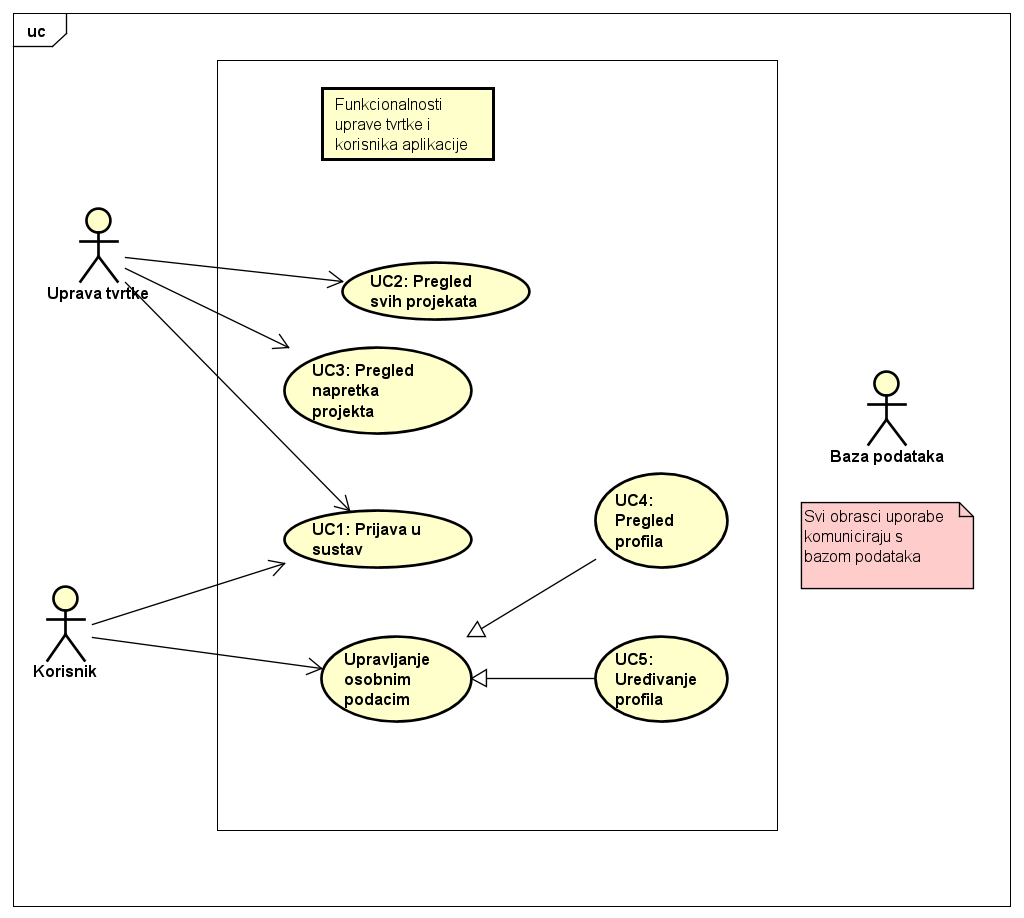
\includegraphics[width=\textwidth]{slike/funkc_korisnika_i_uprave.png}
						\caption{Dijagram obrasca uporabe, funkcionalnosti uprave tvrtke i korisnika}
					\end{figure}
					
					
					\begin{figure} 
						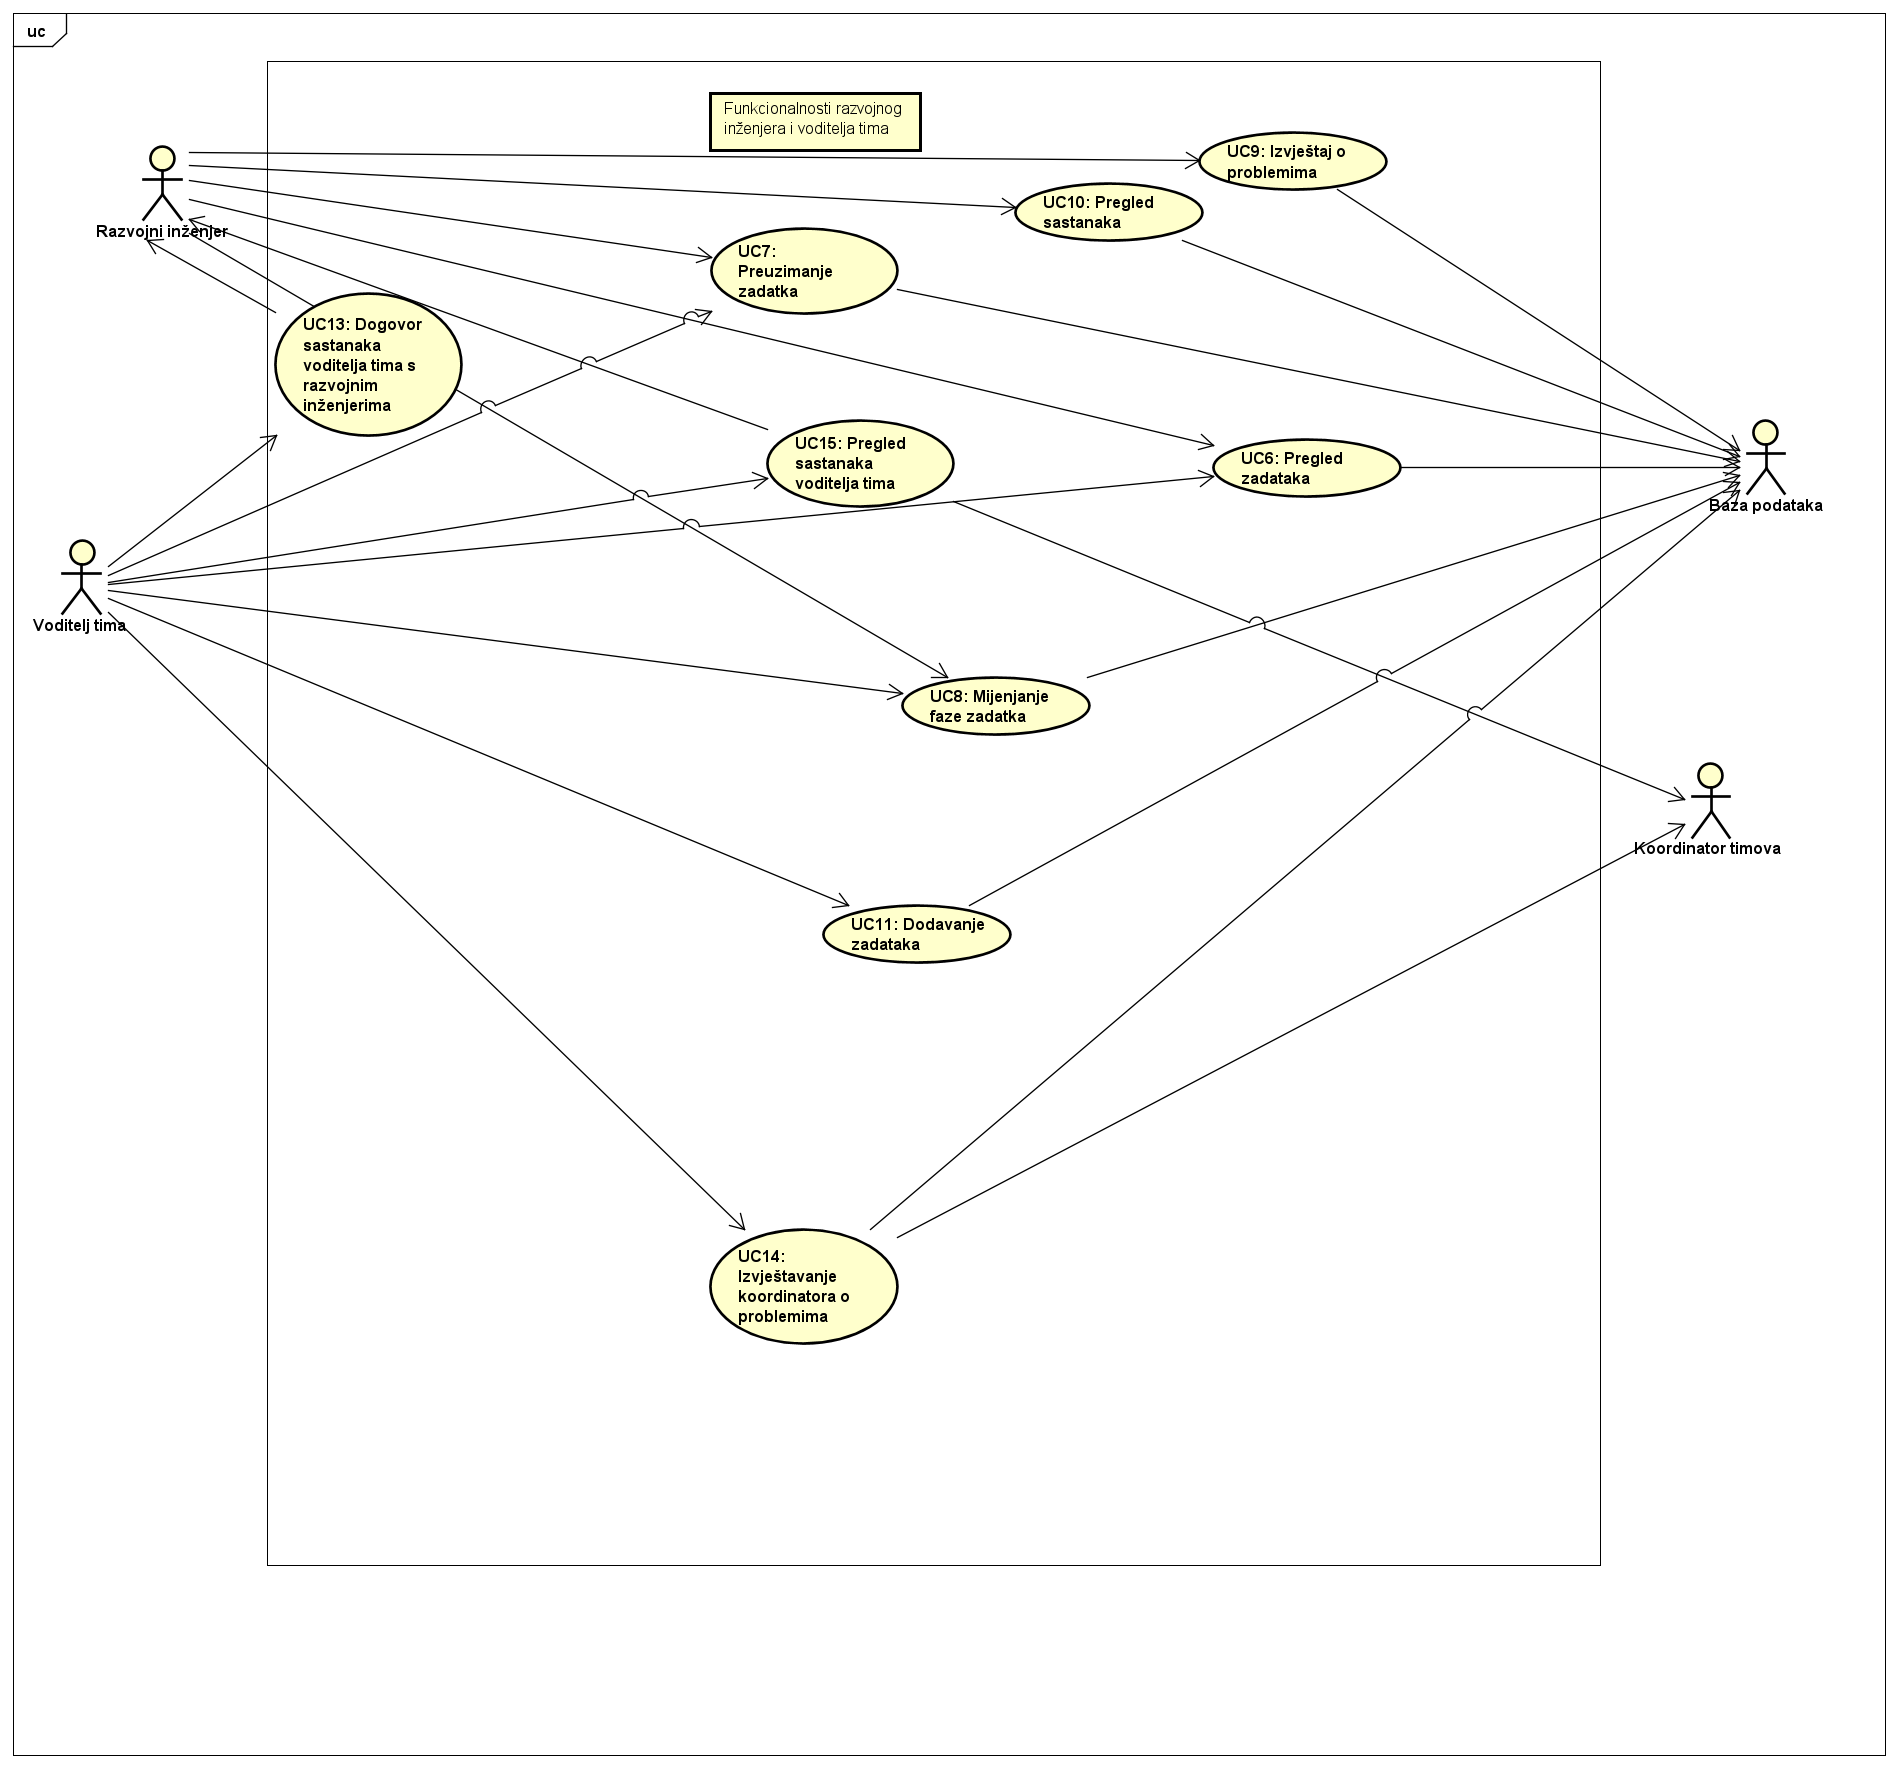
\includegraphics[width=\textwidth]{slike/funkc_razvojnog_inzenjera_i_voditelja.png}
						\caption{Dijagram obrasca uporabe, funkcionalnosti razvojnog inženjera i voditelja tima}
					\end{figure}
					
					\begin{figure} 
						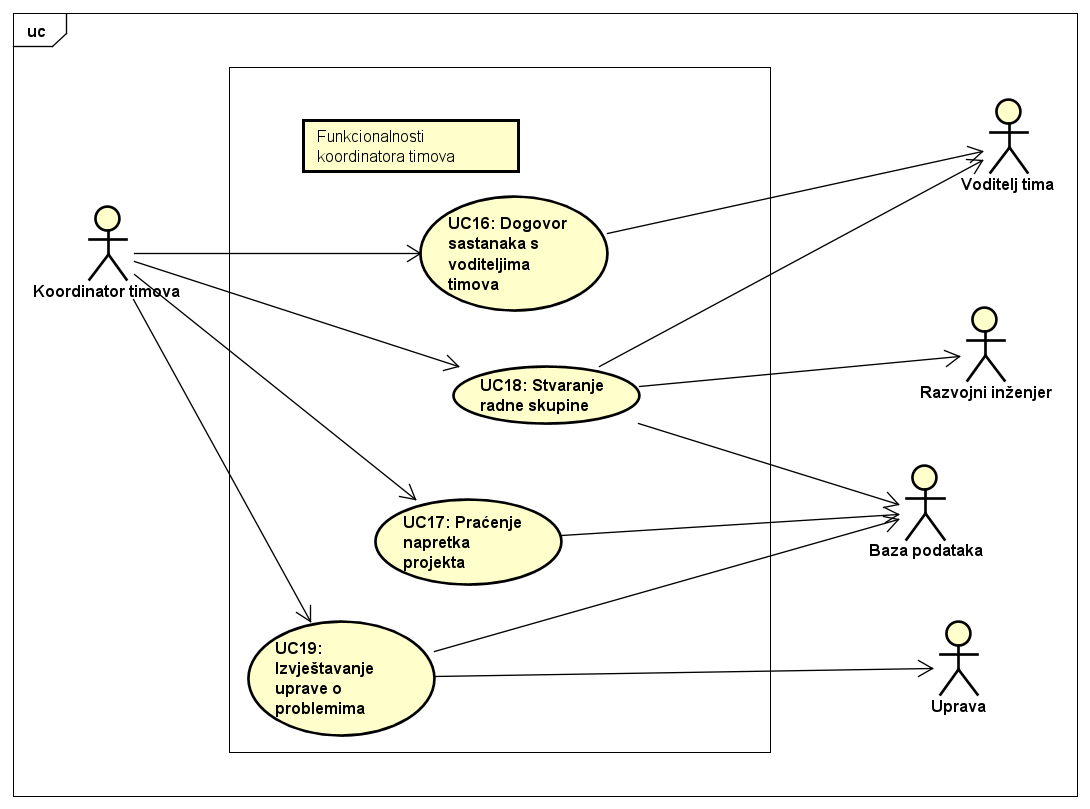
\includegraphics[width=\textwidth]{slike/funkc_koordinatora.png}
						\caption{Dijagram obrasca uporabe, funkcionalnosti koordinatora timova}
					\end{figure}
				\eject		
				
			\subsection{Sekvencijski dijagrami}
				
				\textbf{Obrazac uporabe UC1 - Prijava u sustav}

				\par Član uprave tvrtke unosi korisničko ime i lozinku kako bi se mogao prijaviti u sustav. Poslužitelj pomoću baze podataka provjerava postoji li uneseno korisničko ime i pripada li mu navedena lozinka. Ako su podaci točni članu uprave tvrtke odobrava se ulaz u sustav. Ukoliko podaci nisu ispravni, sustav obavještava člana uprave tvrtke o tome uz poruku. 
				\begin{figure}[h!]
				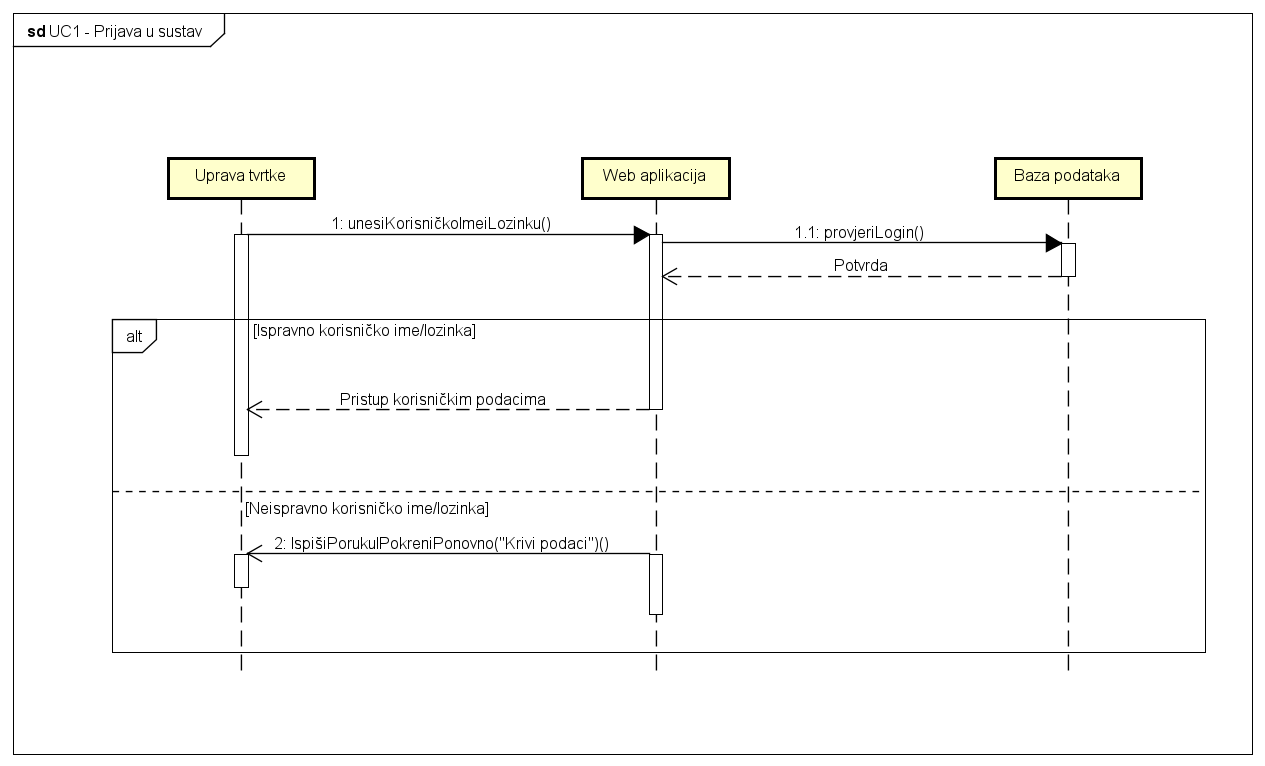
\includegraphics[width=\textwidth]{slike/Sekvencijski_UC1.png}
				\caption{Sekvencijski dijagram za UC1}
				\end{figure}
				\newpage
				\textbf{Obrazac uporabe UC5 - Uređivanje profila}
				
				\par Korisnik traži pristup svojem profilu kako bi ga mogao urediti. Poslužitelj dohvaća korisnikov profil i prikazuje ga. Korisnik na poslužitelju radi promjene prije nego odabere opciju spremanja promjena na profilu. Poslužitelj promjene profila prosljeđuje bazi podataka, a korisnik od poslužitelja traži izlazak iz uređivanja profila. Ukoliko korisnik nije spremio promijenjene podatke, a želi izaći iz uređivanja profila, poslužitelj ga obavještava o tome uz poruku.
				\begin{figure}[h!]
					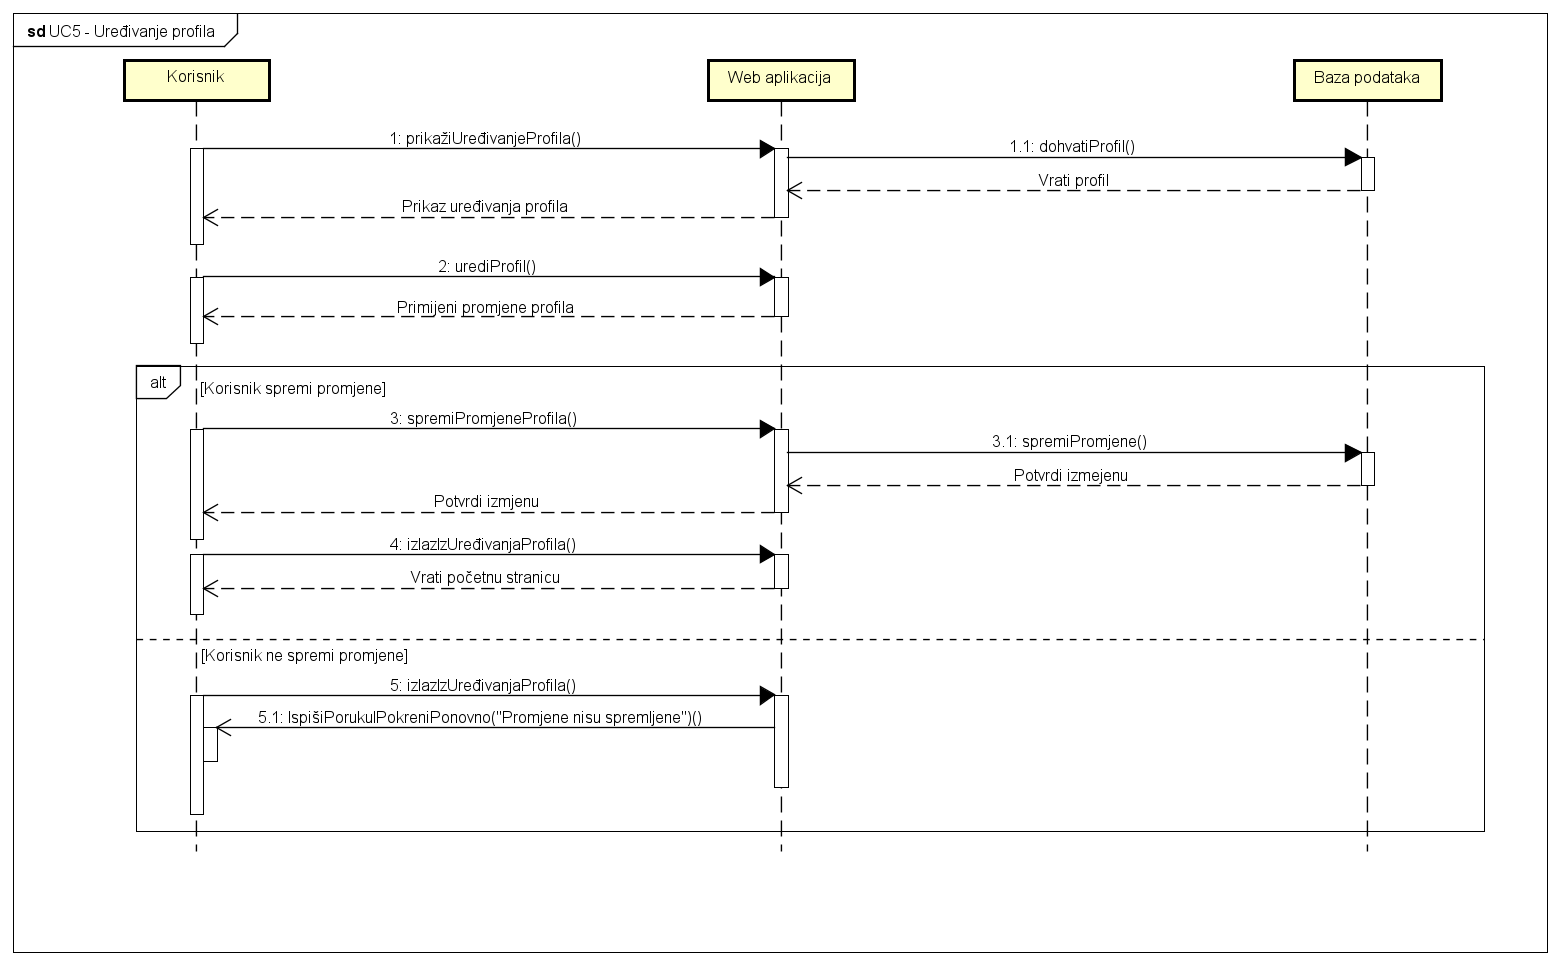
\includegraphics[width=\textwidth]{slike/Sekvencijski_UC5.png}
					\caption{Sekvencijski dijagram za UC5}
					\end{figure}
				\newpage
				\textbf{Obrazac uporabe UC11 - Dodavanje zadataka}
				
				\par Vođa tima odabire opciju za dodavanje novog zadatka. Poslužitelj korisniku vraća obrazac koji on treba popuniti za izradu novog zadatka. Vođa tima na poslužitelju popunjava obrazac za izradu novog zadatka. Vođa tima zatim potvrđuje i sprema novi zadatak. Ukoliko vođa tima nije upisao ime novog zadatka sustav ga obavještava o tome uz poruku. U suprotnom slučaju poslužitelj prosljeđuje novi zadatak u bazu podataka.
				\begin{figure}[h]
					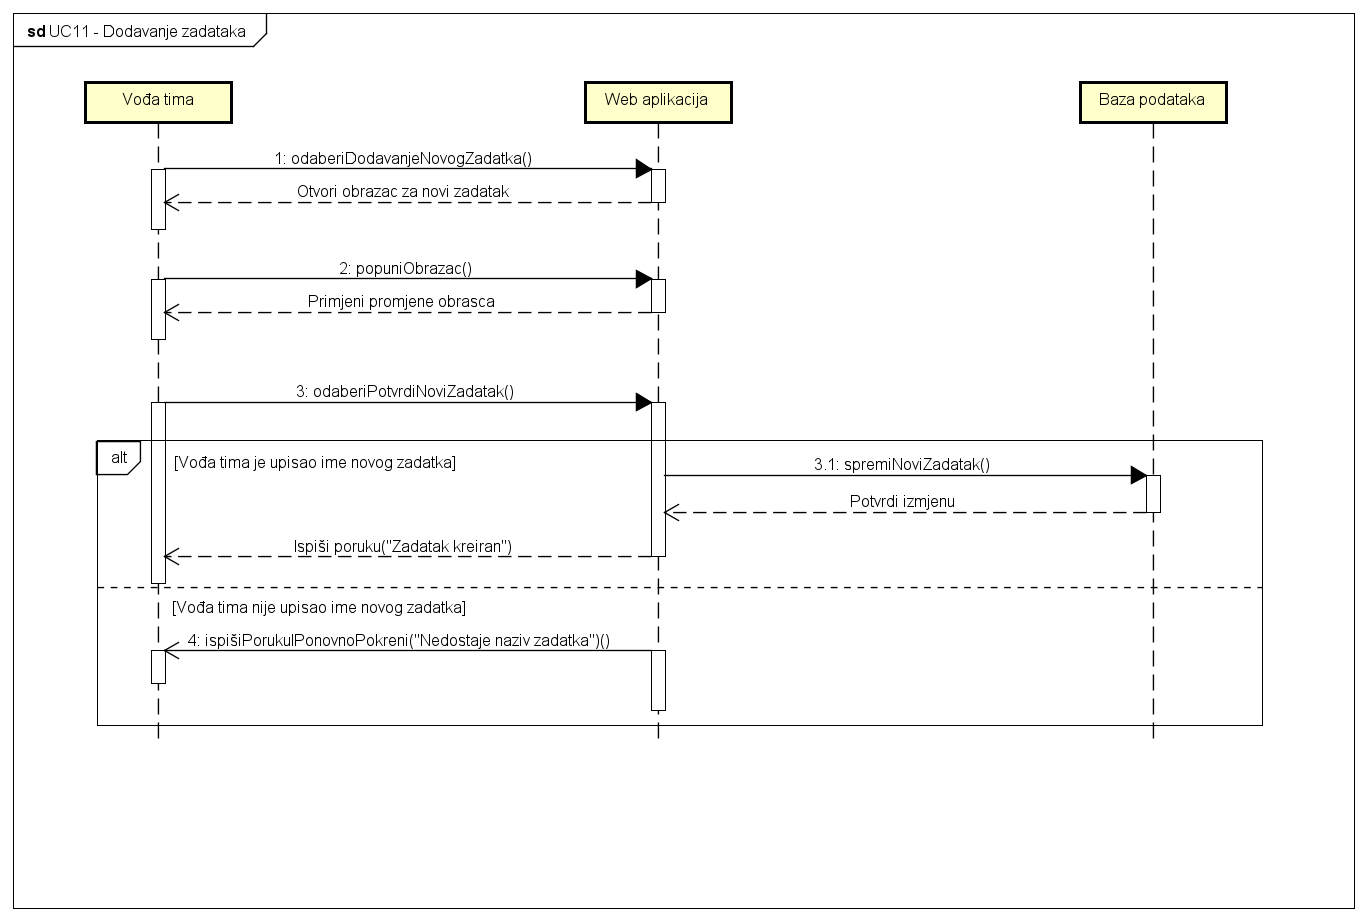
\includegraphics[width=\textwidth]{slike/Sekvencijski_UC11.png}
					\caption{Sekvencijski dijagram za UC11}
					\end{figure}
				\newpage
				\textbf{Obrazac uporabe UC18 - Stvaranje radne skupine}
				
				\par Koordinator traži prikaz radnih grupa. Poslužitelj dohvaća postojeće radne grupe i prikazuje ih. Koordinator  odabire opciju za izradu nove radne skupine zbog čega mu poslužitelj vraća obrazac za izradu nove radne skupine. Korisnik popuni obrazac nakon čega poslužitelj uspoređuje podatke iz obrasca s onima iz baze podataka. Ukoliko koordinator nije upisao ime radne skupine ili nije odabrao tim poslužitelj će ga obavijestiti uz pripadajuću poruku i nastaviti s ispunjavanjem obrasca. Ukoliko je kooordinator odabrao tim koji već pripada radnoj skupini ili je odabrao naziv koji se već koristi, također će biti obaviješten od strane poslužitelja i nastaviti će se s popunjavanjem obrasca. Kada su podaci ispravni koordinator želi napustiti obrazac. Ako je koordinator odabrao opciju spremanja radne skupine, onda ju poslužitelj sprema na bazu podataka. U suprotnom slučaju poslužitelj obaviještava koordinatora da nije spremio novu radnu skupinu.
				\begin{figure}[h]
					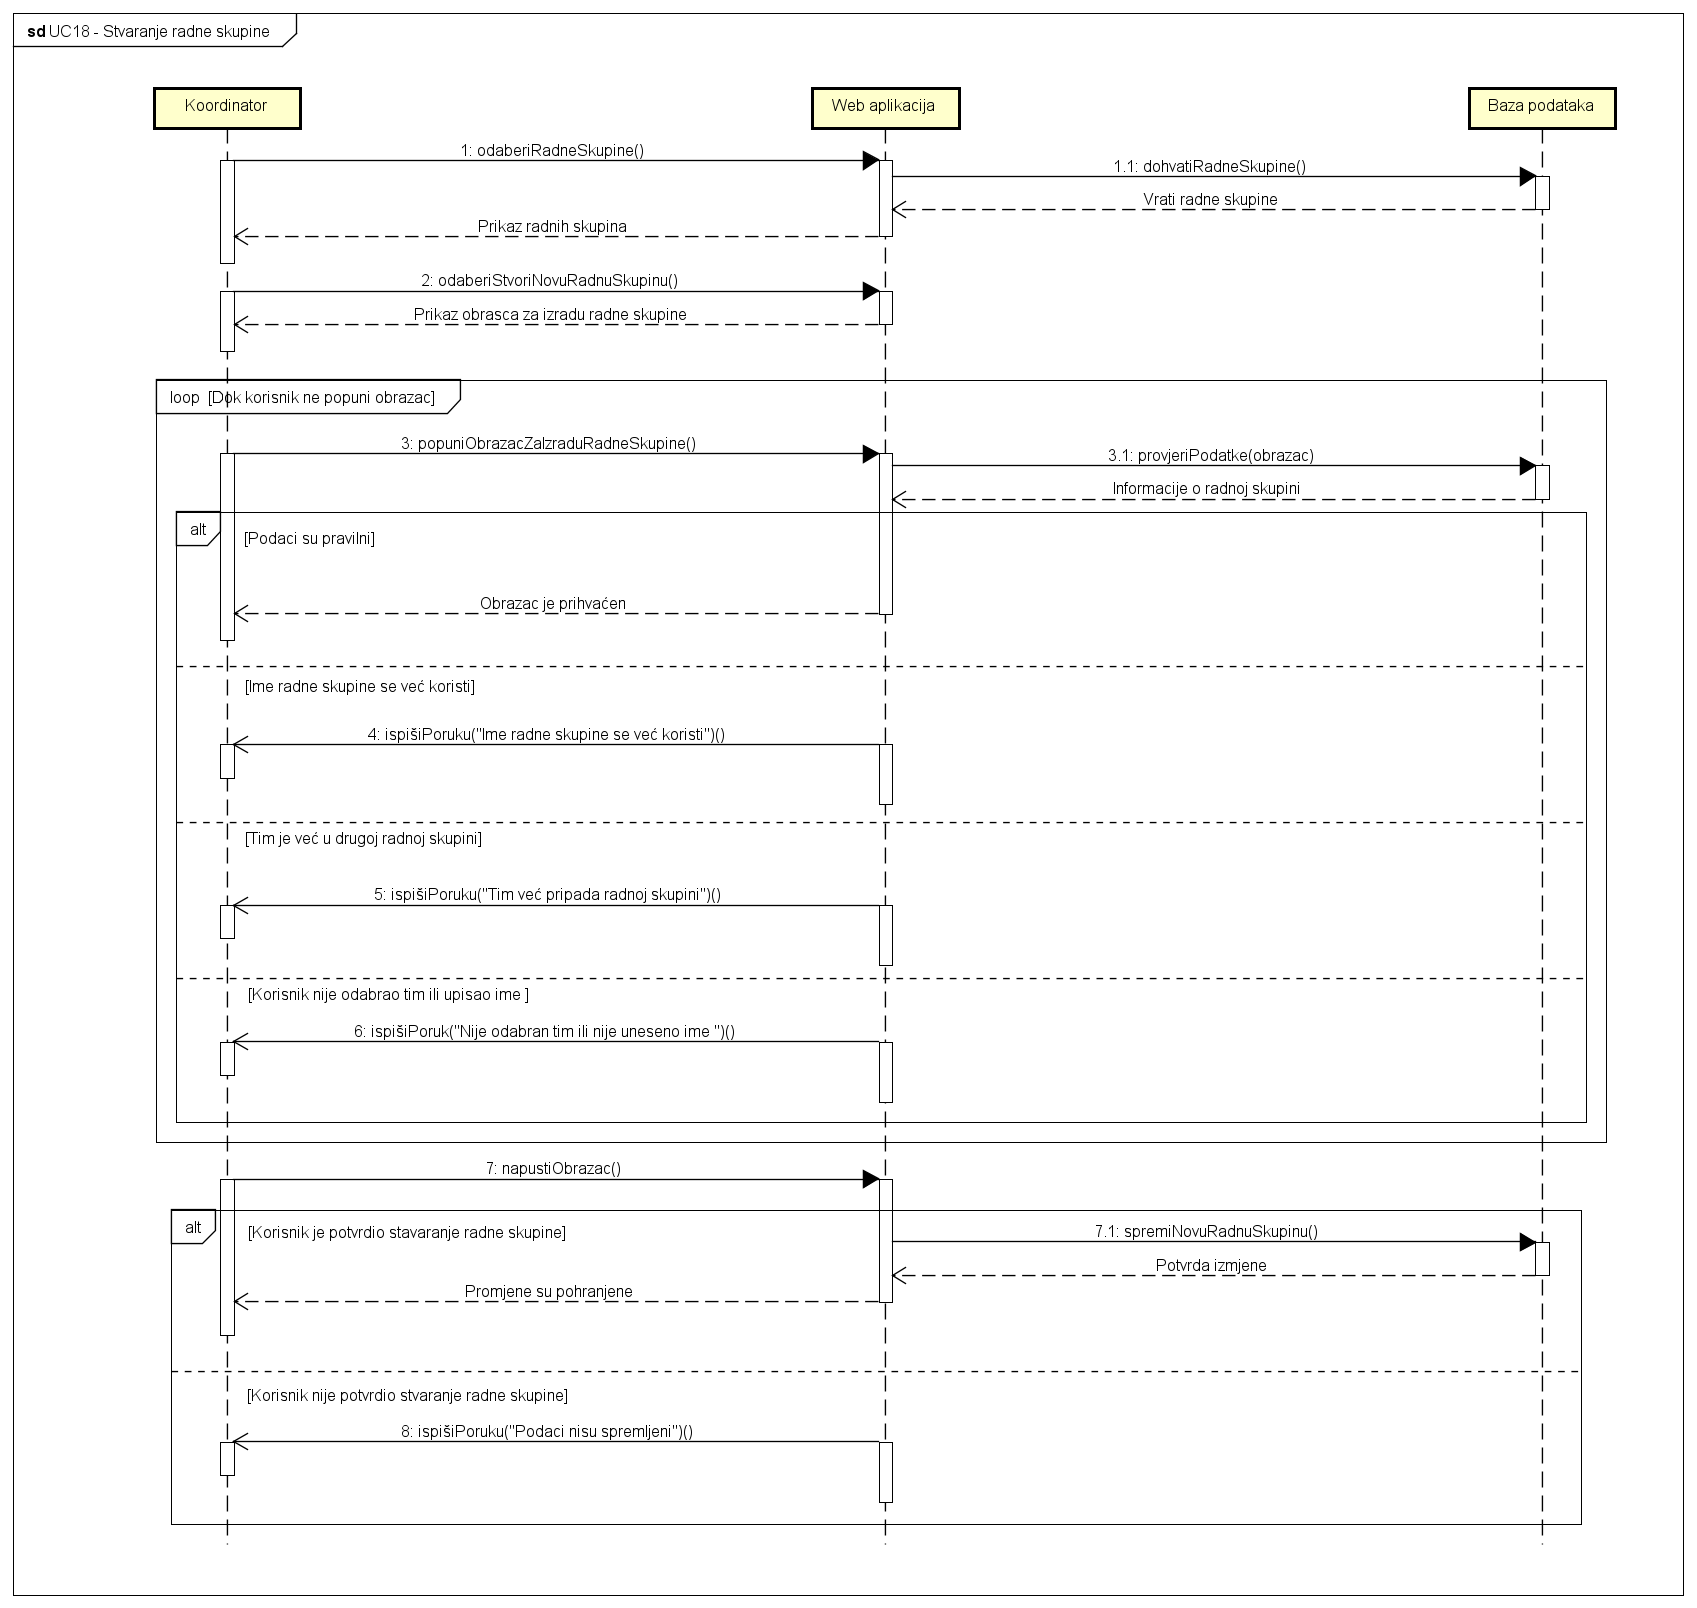
\includegraphics[width=\textwidth]{slike/Sekvencijski_UC18.png}
					\caption{Sekvencijski dijagram za UC18}
					\end{figure}
				\eject
				
		\pagebreak
		\newpage	
		\section{Ostali zahtjevi}
		
			 \begin{itemize}
			 \item Sustav mora podržavati rad za sve zaposlenike tvrtke istovremeno 
			 \item Korisničko sučelje i sustav moraju podržavati hrvatske znakove
			 \item Upiti bazi podataka moraju čekati najviše 3 sekunde
			 \item Sustav treba biti jednostavan i intuitivan za korištenje (KISS princip)
			 \item Sustav mora poštovati načelo nadogradnje uz minimalnu promjenu
			 \item Sustav za raspodjelu zadataka mora koristiti kanban ploču
			 \item za komunikaciju između klijenta i sustava mora biti korišten HTTPS protokol
			 \item veza s bazom podataka mora biti zaštićena, brza i otporna na vanjske greške
			 \item podaci se moraju sanirati prije slanja bazi podataka
			 \end{itemize}
